\documentclass[tikz]{standalone}

\usepackage{ctex}
\usepackage{tikz}
\usepackage{pgfplots}
\pgfplotsset{compat=1.18}   
\usetikzlibrary{positioning, arrows.meta, intersections, calc, fit, backgrounds}
\usepgfplotslibrary{fillbetween}
\begin{document}
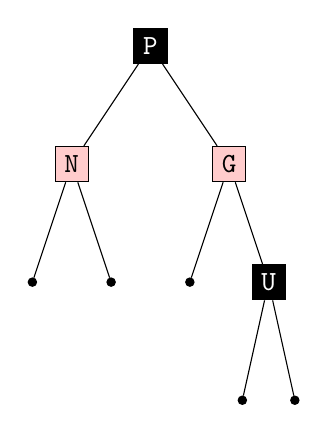
\begin{tikzpicture}[
    % align=center,
    level/.style={sibling distance=2cm/#1},
    every node/.style={draw, font=\ttfamily},
    bnode/.style={fill=black, text=white},
    rnode/.style={fill=red!20},
    nil/.style={circle, draw=black, fill=black, inner sep=0pt, minimum size=3pt},
]

\node[bnode] {P}
    child {node[rnode] {N}
        child {node[nil] {}}
        child {node[nil] {}}
    }
    child {node[rnode] {G}
        child {node[nil] {}}
        child {node[bnode] {U}
            child {node[nil] {}}
            child {node[nil] {}}
        }
    };
\end{tikzpicture}
\end{document}